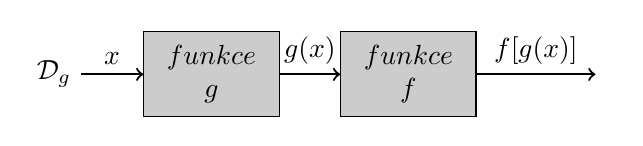
\begin{tikzpicture}[fill=black!20]
%  \draw[help lines] (-1,-2) grid (6,3);
  \path (0,0) node(a) [ ] {\(\mathcal{D}_g\)}
  (2,0) node(b) [rectangle,rotate=0,draw,fill] 
    {\(\begin{array}{c} \text{funkce} \\ g  \end{array}\)}
  (4.5,0) node(c) [rectangle,rotate=0,draw,fill] 
    {\(\begin{array}{c} \text{funkce} \\ f  \end{array}\)}
  (7,0) node(d) [ ] {\(\realset\)};
  \draw[thick,->] (a.east) -- (b);
  \draw[thick,->] (b.east) -- (c);
  \draw[thick,->] (c.east) -- (d);
  \path [ ] (a.east) -- (b.west)   node [above,midway] {\(x\)};
  \path [ ] (b.east) -- (c.west)   node [above,midway] {\(g(x)\)};
  \path [ ] (c.east) -- (d.west)   node [above,midway] {\(f[g(x)]\)};
\end{tikzpicture}